\documentclass{beamer}


\usepackage{graphicx}


\author{Damien DELPY}
\title{Implementation of a Self-Organizing Map}
\institute{ENSEIRB-MATMECA}


\renewcommand{\normalsize}{\fontsize{6}{12}\selectfont}

\setbeamertemplate{footline}{%
	\hfill\insertframenumber/\inserttotalframenumber
}


\begin{document}

\begin{frame}
	
	\titlepage
\end{frame}


\begin{frame}

	\tableofcontents[sectionstyle=show,subsectionstyle=show/shaded/hide,subsectionstyle=show/shaded/hide]
\end{frame}



\section{Overview}
	
	\begin{frame}

		\begin{center}
			
			\Huge OVERWIEW
		\end{center}
	\end{frame}


	\begin{frame}{What is a SOM ?}
		
		\begin{block}{Definition}
 
It is a neural network of just one layer : the output layer.
 	
			
		\begin{center}
			
			\begin{figure}[h]
			
				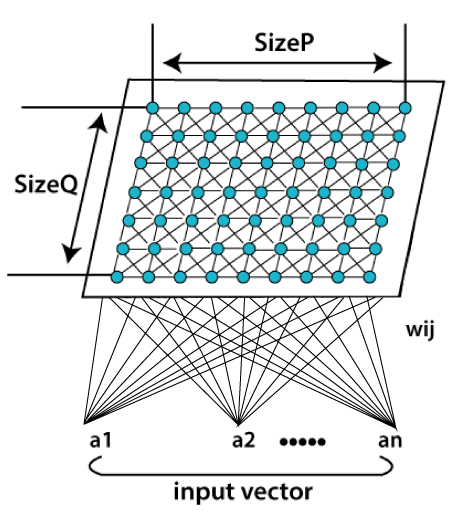
\includegraphics[width=0.3\linewidth]{pics/som_example_diapo_1.png}
				\caption{Representation of a SOM (2 of Bibliography).}
			\end{figure}
		\end{center}

		\end{block}		

		\begin{block}{Wikipedia}

A self-organizing map (SOM) is used to produce a low-dimensional (typically two-dimensional) representation of a higher dimensional data set, while preserving the topological structure of the data. 
		\end{block}
	\end{frame}
	
	
	\begin{frame}{Motivation}

		The Self-Organizing Maps permit to : 

		\begin{itemize}
		
			\item Analyse and visualise the data. It represents complex data on a map of only two or three dimensions (see Convergence slide).

			\item Detect patterns from the data. Clustering (see K-means slide).

			\item Improve a deep neuronal network by sorting the data at the beginning.

		\end{itemize}


	\end{frame}
	
		
	\begin{frame}{Similarities with the Perceptron}
	
		\begin{block}{Perceptron}

			\begin{center}
				
				\begin{figure}[h]

					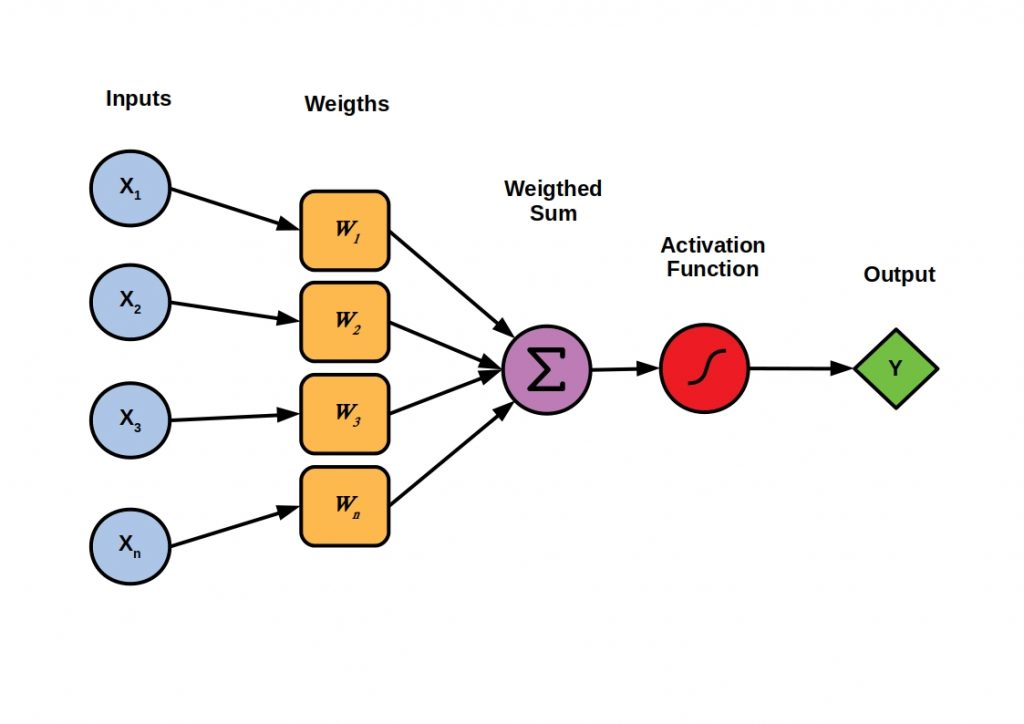
\includegraphics[width=0.4\linewidth]{pics/Perceptrons-1024x724.jpeg}
					\caption{Diagram of a Perceptron.}	
				\end{figure}
			\end{center}

			It is also a one-layer neuronal network. However, this one is used to separate two different classes. The output is actually a binary one. 

			This is a supervised learning algorithm.
		\end{block}

		
		\begin{block}{SOM}
		
			The SOM can gather vectors due to their similarities.

			The SOM is an \textbf{unsupervised learning algorithm}.
		\end{block}



	\end{frame}
	
	
	\begin{frame}{Similarities with K-means algorithm}
		
		K-means algorithm is an unsupervised learning technique that can automatically gather data by creating\textbf{clusters}, which are subsets of data elements that share common characteristics.

		\begin{center}
			
			\begin{figure}[h]
			
				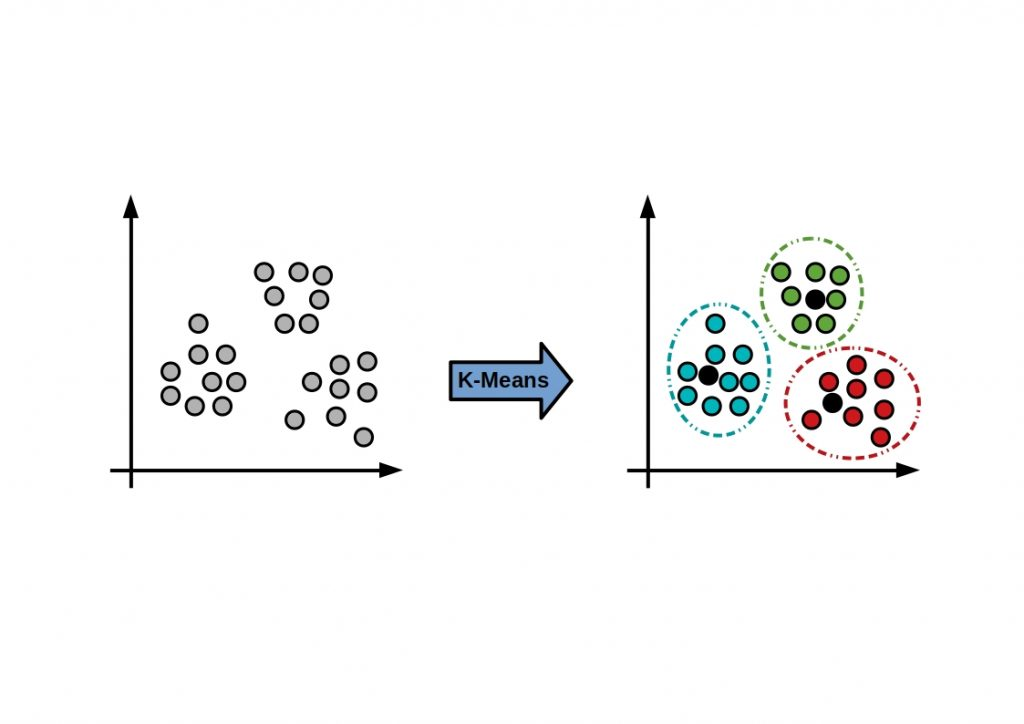
\includegraphics[width=0.6\linewidth]{pics/kmeans.jpeg}
				\caption{Process of K-means algorithm}
			\end{figure}
		\end{center}
				
		The user must define the number of clusters \textbf{K}. However, The SOM does not require this, it guesses the right amount of clusters.

	\end{frame}

	
	\begin{frame}{Convergence}
		
		The convergence of the SOM algorithm is not guaranteed. There are actually 2 errors that can appear.

                     
		\begin{columns}
                        
                        \column{0.5\textwidth}
                
                        	\begin{figure}[h]
                
                                	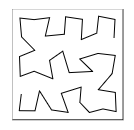
\includegraphics[width=0.5\linewidth]{pics/dimension_error.png}
					\caption{\tiny \textbf{Dimension Error}. 

It happens when the number of neurons does not fit with the data. 

The ideal number of neurons is 5$\sqrt{N}$ where N is the number of data vectors.}
                        	\end{figure}
                        
                        
                        \column{0.5\textwidth}
                        
                        	\begin{figure}[h]
                                
                                	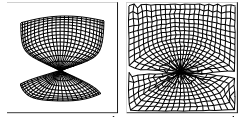
\includegraphics[width=0.5\linewidth]{pics/topological_error.png} 
					\caption{\tiny \textbf{Topological Error}. 

It happens when a node is created. It looks like a butterfly.}             
                        	\end{figure}
		\end{columns}
	\end{frame}



\section{Algorithm}

	\begin{frame}
	
		\begin{center}
			
			\Huge ALGORITHM
		\end{center}
	\end{frame}










\section{Bibliography}
	
	\begin{frame}
	
		\begin{center}

			\Huge BIBLIOGRAPHY
		\end{center}
	\end{frame}


	\begin{frame}
	
		\begin{enumerate}
			
			\item Self-Organizing Maps - Teuvo Kohonen (2001)
			\item https://www.baeldung.com/cs/som-algorithm
			\item http://www.pspc.unige.it/~drivsco/Papers/VanHulle$\textunderscore$Springer.pdf
		\end{enumerate}
	\end{frame}





\end{document}
